\begin{figure*}[htb]
\centering
\subfigure[a] {\label{fig:ite}   \includegraphics[width=0.32\textwidth]{fig/ppw_16_ite.eps}}%
\subfigure[b] {\label{fig:taylor}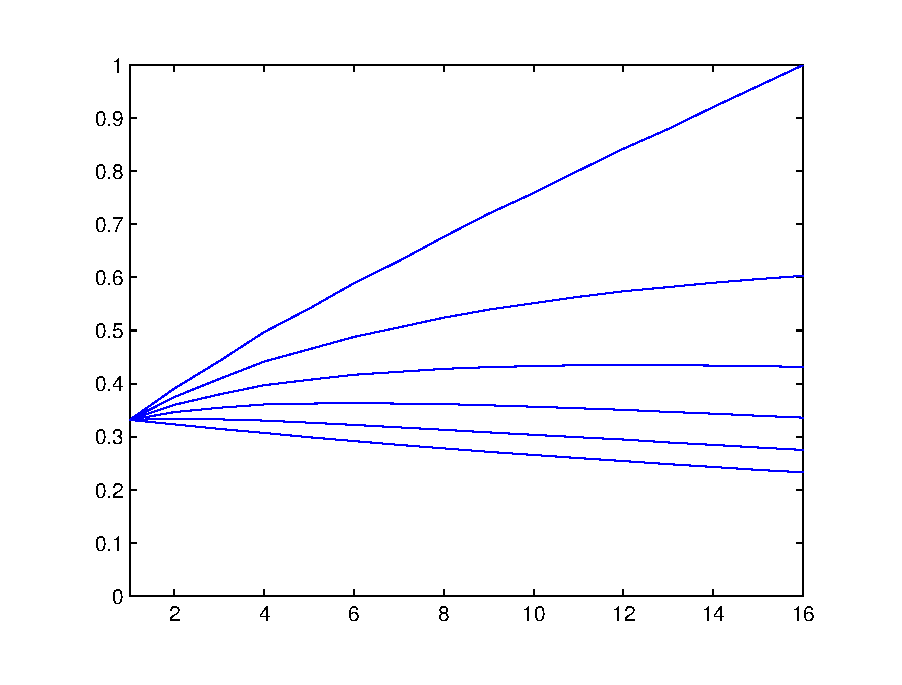
\includegraphics[width=0.32\textwidth]{fig/ppw_16_taylor.eps}}%
\subfigure[c] {\label{fig:tayboo}\includegraphics[width=0.32\textwidth]{fig/ppw_16_tayboo.eps}}
\caption{PPW}  
\label{fig:ppw}
\end{figure*}


\section{Experimental Results}

In this section, we evaluate both accuracy and efficiency of the proposed light core distribution estimation method. All data are collected on a PC with Intel I5 2400 CPU and 3 GB memory. In the experiment, multi-core systems with the number of cores ranging from 9 to 64 are used, and each system is tested with different parallel computation ratios. The thermal models of these systems are extracted from HotSpot [x] with default package and chip parameters. For all test cases, we set the ambient temperature as \SI{20}{\degreeCelsius}, and the thermal constraint as \SI{95}{\degreeCelsius}. 

\subsection{Experiment setup}


Through HSPICE simulation, the impact of temperature on device leakage can be characterized. With the collected data, we can obtain the parameters of model through curve fitting as shown in Fig.x. The ambient temperature is set to be \SI{20}{\degreeCelsius}.

For accuracy and speed comparison, we first perform the iteration based power estimation, which is accurate but very time-consuming, therefore we consider it as the golden accuracy baseline (golden for short). Then, two acceleration methods, the Taylor expansion based method 